
% \section{Grundlagen der Rossby-Wellen}

\begin{frame}{Idealisiertes zonales Windfeld}
	\begin{columns}
		\column{0.55\textwidth}
		\begin{itemize}
			\item Gezeigt ist ein simuliertes \textbf{zonales Windfeld}:
			      \begin{itemize}
				      \item Reine Ost-West-Strömung (\(v = 0\))
				      \item Geschwindigkeit abhängig von der Breite: \(u = U_0 \cdot \sin^2(\theta)\)
				      \item Keine Druckgradienten oder vertikale Struktur
			      \end{itemize}
		\end{itemize}

		\column{0.45\textwidth}
		\centering
		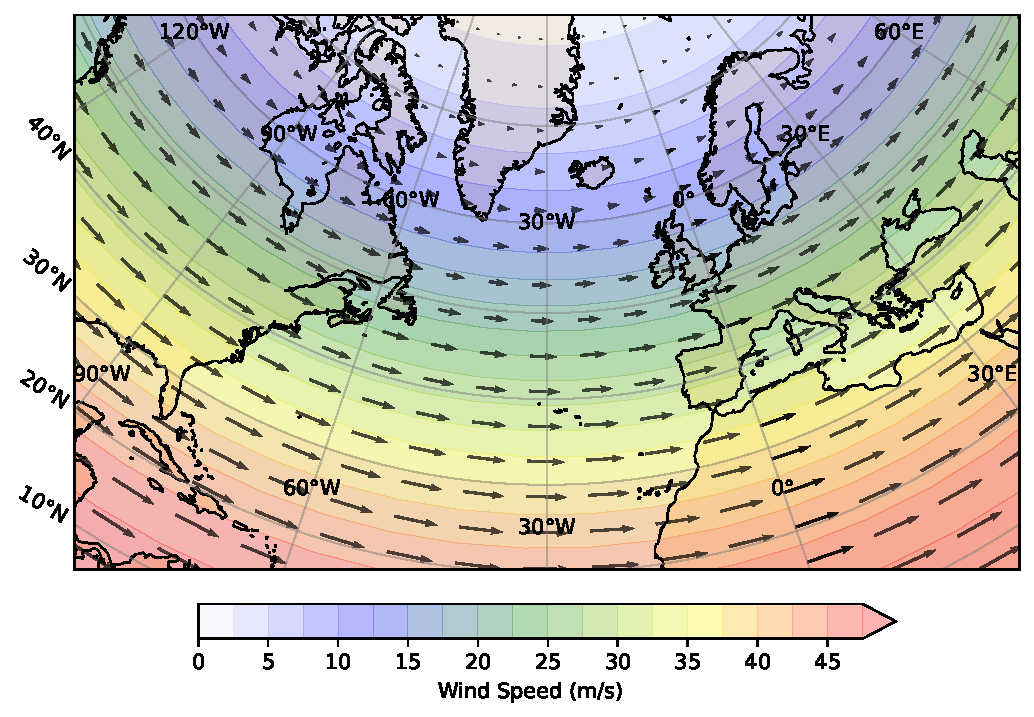
\includegraphics[width=\linewidth]{../images/zonal_wind_plot.pdf}
	\end{columns}
\end{frame}


\begin{frame}{Idealisiertes meridionales Windfeld}
	\begin{columns}
		\column{0.55\textwidth}
		\begin{itemize}
			\item Gezeigt ist ein simuliertes \textbf{meridionales Windfeld}:
			      \begin{itemize}
				      \item Reine Nord-Süd-Strömung (\(u = 0\))
				      \item Geschwindigkeit abhängig von der Breite: \(v = V_0 \cdot \cos(\theta)\)
			      \end{itemize}
		\end{itemize}

		\column{0.45\textwidth}

		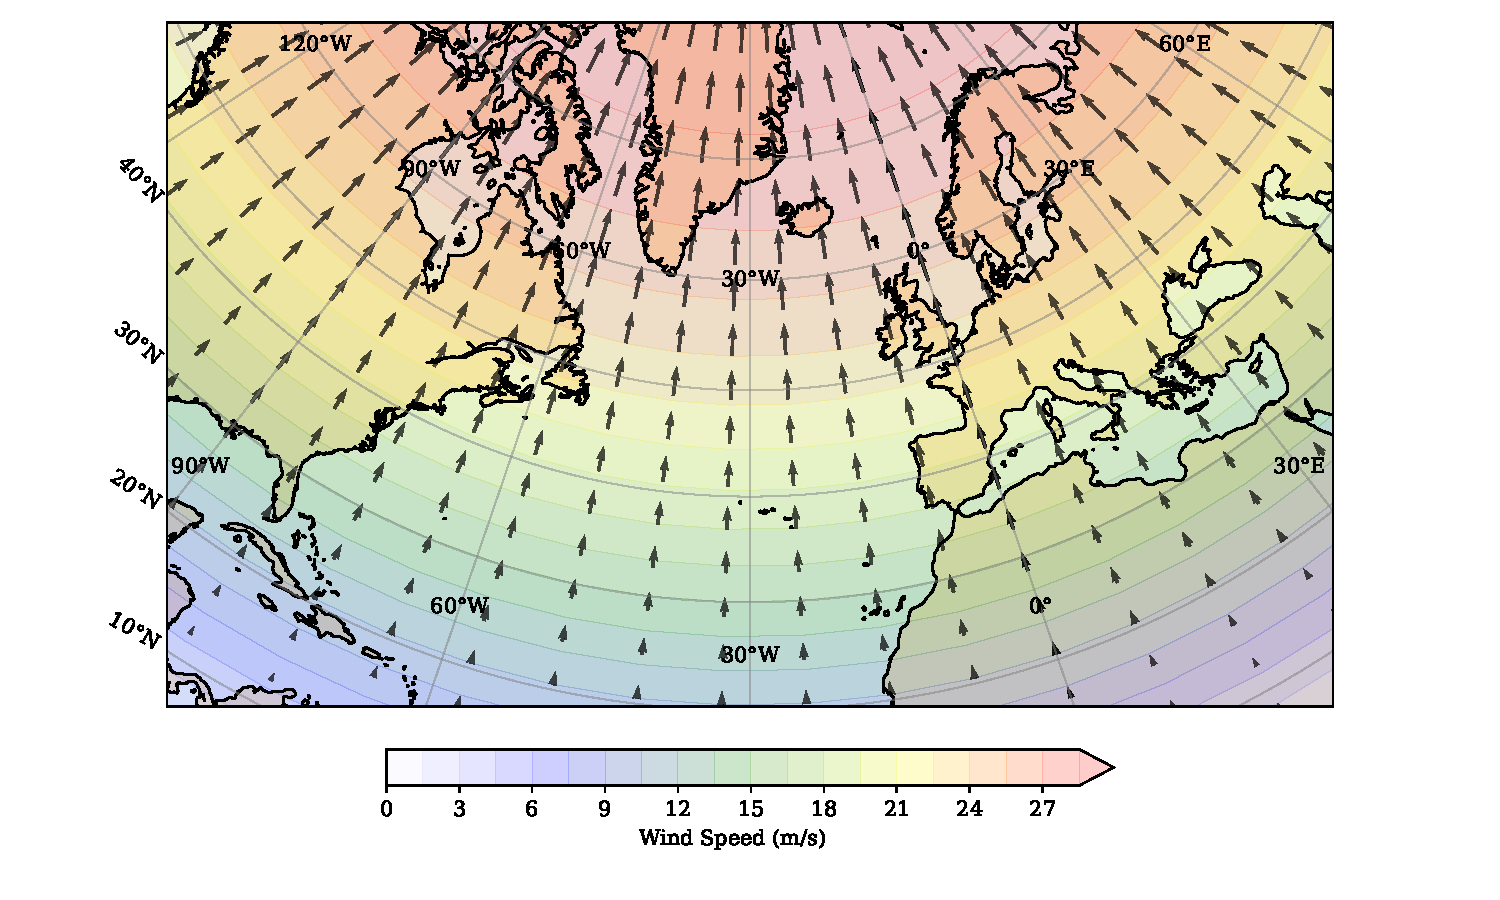
\includegraphics[width=\linewidth]{../images/meridional_wind_plot.pdf}

	\end{columns}
\end{frame}

\foreach \n in {01,02,03,04,05,06,07,08,09,10,
                11,12,13,14,15,16,17,18,19,20,
                21,22,23,24,25,26,27,28,29,30,
                31} {
  \begin{frame}[plain]
    \begin{center}
      \includegraphics[width=0.75\textwidth]{../images/rotating_earth/fig_\n.pdf}
    \end{center}
  \end{frame}
}

\begin{frame}{Corioliskraft: Grundprinzip}
	\begin{itemize}
		\item Die \textbf{Corioliskraft} ist eine Scheinkraft, die in rotierenden Bezugssystemen wie der Erde wirkt.
		\item Sie verursacht eine Ablenkung von bewegten Luft- und Wassermassen:
		      \begin{itemize}
			      \item \textbf{Nordhalbkugel:} Ablenkung nach rechts
			      \item \textbf{Südhalbkugel:} Ablenkung nach links
		      \end{itemize}
		\item Maximale Wirkung an den Polen, null am Äquator.
	\end{itemize}
\end{frame}

\begin{frame}{Mathematische Formulierung}
	\begin{equation*}
		\vec{F}_C = -2m (\vec{\Omega} \times \vec{v})
	\end{equation*}
	\vspace{0.5cm}
	\begin{itemize}
		\item \( m \): Masse des Körpers
		\item \( \vec{\Omega} \): Rotationsvektor der Erde
		\item \( \vec{v} \): Geschwindigkeit relativ zur Erdoberfläche
	\end{itemize}
\end{frame}

\begin{frame}{Beispiel: Corioliskraft beim Velofahren}
	\textbf{Gegeben:}
	\begin{itemize}
		\item Geschwindigkeit: \( \vec{v} = 8.33\,\mathrm{m/s} \) (30 km/h)
		\item Masse: \( m = 80\,\mathrm{kg} \)
		\item Breite: \( \varphi = 47^\circ \) (Zürich)
		\item Erdrotation:
		      \[
			      23\,\mathrm{h}\,56\,\mathrm{min}\,4\,\mathrm{s} \quad\Rightarrow\quad
			      \vec{\Omega} = \frac{2\pi}{86164\,\mathrm{s}} \approx 7.292 \times 10^{-5}\,\mathrm{rad/s}
		      \]
	\end{itemize}

	\vspace{0.3cm}
	\textbf{Formel:}
	\[
		F_C = 2 m \vec{v} \vec{\Omega} \sin(\varphi)
	\]

	\vspace{0.3cm}
	\textbf{Einsetzen:}
	\[
		F_C \approx 2 \cdot 80 \cdot 8.33 \cdot 7.292 \times 10^{-5} \cdot \sin(47^\circ)
		\approx 0.070\, \mathrm{N}
	\]

\end{frame}


\begin{frame}{Breitenabhängigkeit und Coriolis-Parameter}
	\begin{itemize}
		\item Der \textbf{Coriolis-Parameter} beschreibt die Breitenabhängigkeit:
		      \[
			      f = 2 \Omega \sin(\phi)
		      \]
		\item Seine Änderung mit der Breite ergibt den \textbf{\(\beta\)-Parameter}:
		      \[
			      \beta = \frac{\partial f}{\partial y} = \frac{2 \Omega \cos(\phi)}{a}
		      \]
		\item \(a\): Erdradius, \quad \(y\): Nord-Süd-Koordinate
	\end{itemize}
\end{frame}

\begin{frame}{Simulation der Corioliskraft auf Nordströmung}
	\begin{columns}
		\column{0.55\textwidth}
		\begin{itemize}
			\item Darstellung: Ablenkung von Luftpaketen bei rein meridionaler Startgeschwindigkeit (\(v = 1\), \(u = 0\))
			\item Nach \texttt{steps = 100} Zeitschritten:
			      \begin{itemize}
				      \item Auf Nordhalbkugel: Ablenkung nach Osten
				      \item Auf Südhalbkugel: Ablenkung nach Westen
			      \end{itemize}
			\item Breitenabhängigkeit durch \(f = 2 \Omega \sin(\phi)\)
		\end{itemize}

		\column{0.45\textwidth}
		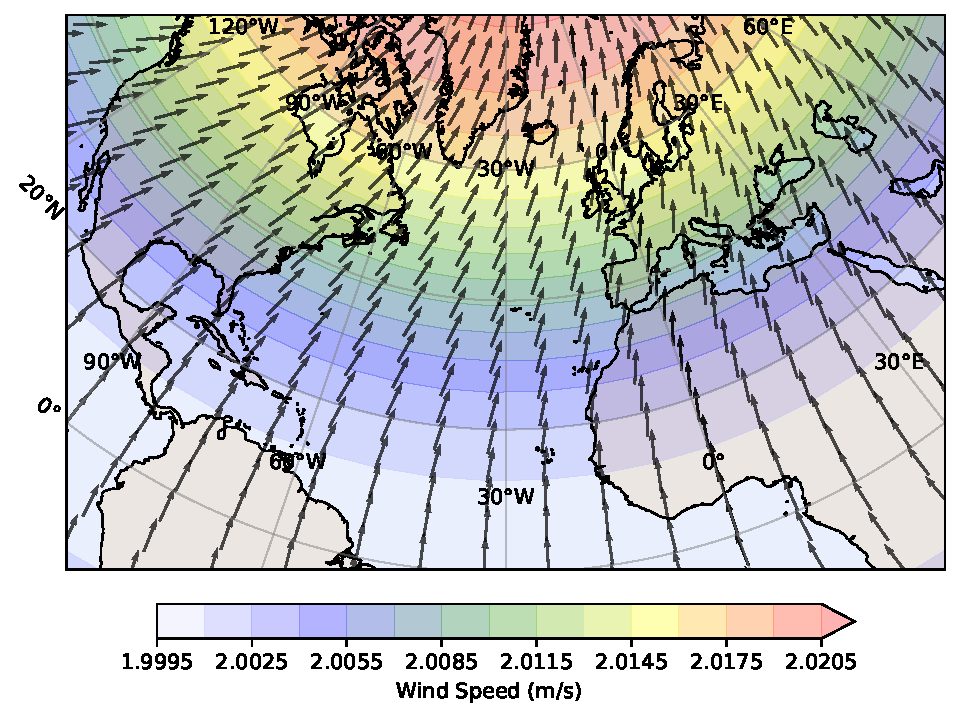
\includegraphics[width=\linewidth]{../images/coriolis_effect_plot.pdf}
	\end{columns}
\end{frame}

% \begin{frame}{Numerische Simulation der Corioliskraft}
% 	\begin{itemize}
% 		\item \textbf{Rotation der Erde:}
% 		      \[
% 			      \Omega = 7.2921 \cdot 10^{-5} \ \text{rad/s}, \quad f = 2 \Omega \sin(\phi)
% 		      \]
% 		      Der Coriolisparameter \( f \) steigt mit der geographischen Breite \(\phi\), ist bei \(\phi = 0^\circ\) null.

% 		\item \textbf{Initialisierung:}
% 		      \[
% 			      v = 1 \, (\text{Nord}), \quad u = 0 \, (\text{Ost}), \quad dx = dy = 0
% 		      \]
% 		      Alle Luftpakete starten mit rein meridionaler Geschwindigkeit.

% 		\item \textbf{Zeitschritte:} (Euler-Verfahren)
% 		      \[
% 			      u_{t+1} = u_t + f \cdot v_t \cdot \Delta t,\quad
% 			      v_{t+1} = v_t - f \cdot u_t \cdot \Delta t
% 		      \]
% 		      \[
% 			      dx += u_{t+1} \cdot \Delta t,\quad dy += v_{t+1} \cdot \Delta t
% 		      \]
% 		      Die Bewegung wird durch die Corioliskraft kontinuierlich abgelenkt.
% 	\end{itemize}
% \end{frame}


\begin{frame}
	\frametitle{$\beta$-Ebene Approximation}
	\begin{center}
		\begin{tikzpicture}[scale=2]
			% Tilted group (Earth and axes)
			\begin{scope}[rotate around={23.5:(0,0)}]
				% Axes
				\draw (-2,0) -- (2,0);
				\draw[->] (0,-2) -- (0,2) node[above] {$Pole$};

				% Earth (circle)
				\draw[thick] (1,0) arc[start angle=0, end angle=360, radius=1];

				% 3D-style spinning arrow (elliptical path)
				\draw[->, thick] ({0.3*cos(10)},{1.5 + 0.1*sin(10)})
				arc[start angle=10, end angle=320, x radius=0.3, y radius=0.1];
				% Point on the circle
				% \fill[red] ({cos(20)}, {sin(20)}) circle[radius=0.05] node[below right] {$P$};
				\fill[red] (30:1) circle[radius=0.05] node[right] {$P$};
				\draw[blue, thick] ($(30:1) + (120:0.5)$) -- ($(30:1) + (-60:0.5)$);
			\end{scope}
		\end{tikzpicture}
	\end{center}
\end{frame}


% \begin{frame}{Bedeutung für Rossby-Wellen}
% 	\begin{itemize}
% 		\item Rossby-Wellen entstehen durch:
% 		      \begin{itemize}
% 			      \item Erhaltung der absoluten Vorticity
% 			      \item Variation der Corioliskraft mit der Breite (\(\beta\)-Effekt)
% 		      \end{itemize}
% 		\item Bewegung nach Norden: Zunahme von \(f\), erzeugt zyklonale Vorticity
% 		\item Rückstellende Wirkung → wellenartige Westwärts-Ausbreitung
% 	\end{itemize}
% \end{frame}

% \begin{frame}{Fazit}
% 	\begin{itemize}
% 		\item Die Corioliskraft lenkt Luftmassen ab und hängt von der geographischen Breite ab.
% 		\item Ihre Breitenänderung ist die physikalische Grundlage für Rossby-Wellen.
% 		\item Ohne Corioliskraft gäbe es keine grossskaligen planetaren Wellen wie Jetstreams.
% 	\end{itemize}
% \end{frame}

\begin{frame}{Was ist die \(\beta\)-Ebene?}
	\begin{itemize}
		\item Die \textbf{\(\beta\)-Ebene} ist eine lokale Approximation der Erdkugel nahe einer bestimmten Breite \(\phi_0\).
		\item Ziel: Vereinfachung der Corioliskraft für mathematische Modelle.
		\item Der Coriolisparameter \(f\) wird linearisiert:
		      \[
			      f(y) = f_0 + \beta y
		      \]
		      mit:
		      \begin{itemize}
			      \item \(f_0 = 2\Omega \sin(\phi_0)\): Coriolisparameter an der Referenzbreite
			      \item \(\beta = \left.\frac{\partial f}{\partial y}\right|_{\phi_0} = \frac{2\Omega \cos(\phi_0)}{a}\)
			      \item \(y\): meridionale Entfernung vom Referenzbreitenkreis
		      \end{itemize}
	\end{itemize}
\end{frame}

% \begin{frame}{Warum ist die \(\beta\)-Ebene wichtig?}
% 	\begin{itemize}
% 		\item Ermöglicht analytische Lösungen für Rossby-Wellen:
% 		      \[
% 			      \text{Wellengleichung:} \quad \frac{\partial \zeta}{\partial t} + \beta v = 0
% 		      \]
% 		\item Führt zur Dispersionsrelation für barotrope Rossby-Wellen:
% 		      \[
% 			      \omega = -\frac{\beta k}{k^2 + l^2}
% 		      \]
% 		\item Die Wellen bewegen sich \textbf{westwärts}, auch wenn der Wellenvektor ostwärts zeigt!
% 	\end{itemize}
% \end{frame}

% \begin{frame}{Zusammenfassung \(\beta\)-Ebene}
% 	\begin{itemize}
% 		\item Lokale Näherung, um Breitenabhängigkeit von \(f\) zu berücksichtigen.
% 		\item Ideal für theoretische Untersuchungen von grossskaliger Dynamik.
% 		\item Grundlage für das Verständnis von Rossby-Wellen, atmosphärischer Stabilität und grossräumiger Zirkulation.
% 	\end{itemize}
% \end{frame}

% \begin{frame}{Vorticity – Wirbelstärke in der Atmosphäre}
% 	\begin{itemize}
% 		\item \textbf{Relative Vorticity} \(\zeta\): Rotation der Strömung relativ zur Erde
% 		      \[
% 			      \zeta = \frac{\partial v}{\partial x} - \frac{\partial u}{\partial y}
% 		      \]
% 		\item \textbf{Absolute Vorticity} \(q\): Summe aus relativer Vorticity und planetarer Vorticity
% 		      \[
% 			      q = \zeta + f
% 		      \]
% 		\item \textbf{Satz zur Erhaltung der absoluten Vorticity} (ohne Reibung):
% 		      \[
% 			      \frac{D}{Dt} (\zeta + f) = 0
% 		      \]
% 	\end{itemize}
% \end{frame}

% \begin{frame}{Physikalische Interpretation}
% 	\begin{itemize}
% 		\item Ein Luftpaket, das sich in meridionaler Richtung bewegt, erlebt Änderung in \(f\).
% 		\item Um die totale Vorticity konstant zu halten, ändert sich \(\zeta\) – es wird zyklonaler oder antizyklonaler.
% 		\item \textbf{Das erzeugt eine rückstellende Kraft} → wellenförmige Bewegung entsteht.
% 	\end{itemize}

% 	\vspace{0.4cm}
% 	\textbf{Dies ist die physikalische Grundlage der Rossby-Wellen!}
% \end{frame}

% \begin{frame}{Linearisierte Vorticity-Gleichung (auf \(\beta\)-Ebene)}
% 	\begin{itemize}
% 		\item Wir betrachten kleine Störungen \(u', v'\) über einer zonalen Grundströmung \(U\).
% 		\item Einsetzen in die Vorticity-Gleichung ergibt:
% 		      \[
% 			      \frac{\partial}{\partial t} (\nabla^2 \psi') + U \frac{\partial}{\partial x} (\nabla^2 \psi') + \beta \frac{\partial \psi'}{\partial x} = 0
% 		      \]
% 		\item Dabei ist \(\psi'\) das Stromfunktion-Störungsfeld:
% 		      \[
% 			      u' = -\frac{\partial \psi'}{\partial y}, \quad v' = \frac{\partial \psi'}{\partial x}
% 		      \]
% 	\end{itemize}
% \end{frame}

% \begin{frame}{Dispersionsrelation für barotrope Rossby-Wellen}
% 	\begin{itemize}
% 		\item Lösung mit Wellenansatz: \(\psi' \propto e^{i(kx + ly - \omega t)}\)
% 		\item Einsetzen ergibt die Dispersionsrelation:
% 		      \[
% 			      \omega = Uk - \frac{\beta k}{k^2 + l^2}
% 		      \]
% 		\item \textbf{Folge:} Rossby-Wellen bewegen sich in einem ruhenden System stets \textbf{westwärts} (wenn \(U = 0\)).
% 	\end{itemize}
% \end{frame}

% \begin{frame}{Zusammenfassung}
% 	\begin{itemize}
% 		\item Die \textbf{Corioliskraft} nimmt mit der Breite zu → \(\beta\)-Effekt.
% 		\item Die \textbf{absolute Vorticity} ist entlang eines Stromfadens erhalten.
% 		\item Kleine Störungen führen zu \textbf{planetaren Wellen} mit westwärts gerichteter Ausbreitung.
% 		\item Diese Wellen heissen \textbf{Rossby-Wellen} und sind fundamental für die grossräumige atmosphärische Dynamik.
% 	\end{itemize}
% \end{frame}


